%%%%%%%%%%%%%%%%%%%%%%%%%%%%%%%%%%%
%%%% INTRODUCCIÓN A LA MEMORIA %%%%
%%%%%%%%%%%%%%%%%%%%%%%%%%%%%%%%%%%

%Buenos días, mi nombre es Miguel González Moreno, soy un antiguo estudiante de la promoción 2014-2019 de ADE+ITI en la Universidad de Deusto. La memoria de mi proyecto de fin de grado la desarrollé en LATEX y a raíz de dicha memoria se ha creado esta plantilla. La plantilla persigue el objetivo de ayudar a cualquier futuro estudiante que se quiera adentrar en este sistema de procesamiento de textos (LATEX). Intentaré explicar cada uno de los campos que aparecen a continuación de modo que todos estén lo más claros posibles y que así, la plantilla, sea de la mayor utilidad posible. Dicho lo cual, comenzamos. 

%Concretamente la memoria y esta plantilla se han realizado en OVERLEAF, un editor de LATEX online pero existen numerosos otros programas que pueden usarse para escribir en este lenguaje. Sin embargo, es posible que algunos de los comandos o funciones cambien de un programa a otro por lo que en caso de cambiar de programa, es probable que algunos comandos no se ejecuten como deberían. En cualquier caso, utilizar otro programa no parece excesivamente complicado pues en caso de que algunos comandos cambien se pueden encontrar fácilmente los equivalentes por Internet. Es cuestión de dedicarle un poco más de tiempo.

%Lo primero de todo, dejar claro que en absoluto soy un experto, es más, ni si quiera soy principiante. Todo lo incluido en esta plantilla se ha aprendido desde cero y lo más probable es que aquello que no está en la plantilla (o que pudiese estar hecho de mejor forma) no lo está puesto que actualmente desconozco como hacerlo, y no porque LATEX no pueda, ya que lo más seguro es que sí se pueda realizar. Así, explicaré todo aquello que sepa dejándoles de profundización en ciertas cuestiones a ustedes. Aquello que desconozca me limitaré a no comentarlo.

%Como se puede observar al compilar, estos textos que aparecen en azul no se escriben en el documento, son comentarios. Los comentarios no son procesados sin embargo sí que se pueden leer en la pantalla de escritura. Intentaré explicar el proceso de creación de la memoria a partir de estos comentarios, siendo todos ellos suprimibles en cuanto el alumno haya comprendido la idea detrás de cada uno de ellos.

%Aún así, si existiese cualquier duda con respecto a la plantilla o a las funciones utilizadas, mi única y principal fuente de conocimiento ha sido Internet, y los maravillosos (y diversos) blogs que se encuentran en la red. Os dejo a continuación aquellos que más me han servido de ayuda (pero la verdad es que hay infinidad). Cualquier función que busquéis, existe. Cualquier problema, lo ha tenido antes otra persona y ha preguntado por ello. Simplemente hay que tener tiempo para encontrar la fuente e ir probando. Esto es prueba y error. 

%Blogs de utilidas: 
%http://minisconlatex.blogspot.com/
%https://tex.stackexchange.com/
%http://metodos.fam.cie.uva.es/~latex/index.html

%Consejo: Por lo general, buscad la ayuda en inglés, hay muchísima más información.

%Finalizada la presentación de la plantilla ¡EMPEZAMOS CON LATEX!

%%%%%%%%%%%%%%%%%%%%%%%%%%%%%%%%
%%%% INTRODUCCIÓN AL LATEX %%%%%
%%%%%%%%%%%%%%%%%%%%%%%%%%%%%%%%

%La escritura en LATEX muy sencilla (una vez se domine lo básico) pero es necesario invertir tiempo para comprenderla, para conocer las funciones y sobre todo para profundizar en ella. Lo básico se aprende rápido. ¡Vamos a ello!

%LATEX trabaja con funciones, todas aquellas palabras que aparecen en verde y van precedidas por el símbolo "\". Cada función suele tener una serie de parámetros opcionales, que se encuentran dentro de "[corchetes]", y una serie de parámetros obligatorios, que se encuentran dentro de "{llaves}". Lógicamente, siempre habrá que introducir un parámetro obligatorio. Los parámetros opcionales se añaden para modificar o precisar elementos de la función en cuestión (dependiendo del uso que le quiera dar el autor).

%En general hay unas funciones básicas que se pueden llamar por defecto, sin embargo para otras es necesario cargar/incluir algunos paquetes especiales. Lo veremos a posteriori (simplemente tenerlo en cuenta).

%%%%%%%%%%%%%%%%%%%%%%%%%
%%%% PRIMERA FUNCIÓN %%%%
%%%%%%%%%%%%%%%%%%%%%%%%%

\documentclass[a4paper,openright,10pt]{book}

%Esta es la primera función del archivo y define el tipo de documento sobre le que se está trabajando. Realmente no tengo un conocimiento exhaustivo sobre los diferentes tipos de documentos en los que se puede trabajar pero encontrar información sobre esta función es muy sencillo.  En este caso, el tipo utilizado es "Book". Se ha utilizado este tipo porque es el más adecuado a documentos largos, con capítulos, secciones y demás. Hay otras clases de documentos como por ejemplo "article", "report" o "memoir". Cada uno con sus características propias. 

%El tipo book permite llamar a otros archivos etcétera. ¿A qué me refiero con llamar a archivos? Como veis en la izquierda estamos trabajando sobre un archivo ".tex" denominado "MAIN.tex". Este archivos es el cuerpo central de nuestra memoria, sin embargo, en él no escribiremos todos los capítulos sino que los capítulos los escribiremos en otros archivos ".tex" (1.Intro.tex, 2.Objetivos.tex y sucesivos) y se llamarán desde "MAIN". Lo veremos más adelante, no os preocupéis. Esto es simplemente para llevar un mayor orden en el documento. Se podría perfectamente escribir toda la memoria en este mismo archivo pero sería algo más caótico y tardaría demasiado en cargar.

%Esta función presntada tiene varios parámetros adicionales: "a4paper", el cual indica que el folio será del tamaño A4, "openright", el cual es utilizado para garantizar que los capítulos nuevos siempre empiecen en una página de la derecha (si en algún momento fuesen a empezar en una página izquierda, LATEX dejará una página en blanco para garantizar esta regla), "10pt" indica el tamaño predeterminado de la fuente a utilizar. 

%Se han indicado así 3 parámetros adicionales. Si no se indican todos los que hay LATEX cogerá los parámetros por defecto en su configuración. Así, que únicamente se hayan indicado 3 no significa que sólo haya 3, probablemente hay muchos más en los que sí se quiere, se puede profundizar buscando información.

%%%%%%%%%%%%%%%%%%%%%%%%%%%%%%%%
%%%% DEFINICIÓN DE PAQUETES %%%%
%%%%%%%%%%%%%%%%%%%%%%%%%%%%%%%%

%LATEX, como se comentaba, no tiene cargadas todas las funciones por defecto (viene lo básico, pero se puede profundizar tanto como se quiera). Así, para ejecutar algunas funciones o símbolos es necesario que se incluyan algunos PAQUETES adicionales. Aquellos en los que se indica PAQUETEB son paquetes prácticamente de inicio, que toda memoria debería como mínimo tener (el resto varía según las necesidades de cada autor).

%Los paquetes se cargan con la función "\usepackage" y aquellos que se han utilizado en la memoria son los siguientes:

\usepackage[utf8]{inputenc}
%PAQUETEB para incluir acentos al escribir en Castellano.
\usepackage[spanish,es-tabla]{babel}
%PAQUETEB para escribir en castellano.
\usepackage{fancyhdr}
%PAQUETEB para definir encabezado y pie de páginas.
\usepackage{ragged2e}
%PAQUETEB utilizado para alinear, justificar o centrar el texto de la memoria.
\usepackage{setspace}
%PAQUETEB para delimitar el interlineado del texto.
%\usepackage{cite}

\usepackage[%
  bibstyle=ieee,
  citestyle=numeric,
  isbn=true,
  doi=false,
  sorting=none,
  url=true,
  defernumbers=true,
  bibencoding=utf8,
  backend=biber
]{biblatex} 

\addbibresource{Bib/MiBiblioteca.bib}


%PAQUETEB para citar y referencia a lo largo del texto.
\usepackage{enumerate} 
%PAQUETEB para formar listas organizadas y darles formato. 
\usepackage[font={color=RBlue},figurename=Fig.]{caption} 
%Paquete para poner subtítulos a las imágenes y concretamente personalizado para que sean de colo azul (elección personal).
\usepackage{graphicx} 
%Paquete para utilizar distintos colores tanto en la escritura, como en tablas, títulos y demás.
\usepackage{subfigure} 
%Paquete para incluir sub-figuras.
\usepackage{hyperref} 
%Paquete para incluir hyperlinks en el PDF.
\usepackage{eurosym} 
%Paquete para incluir el símbolo "€" en el texto.
\usepackage{pdfpages} 
%Paquete para incluir PDFs a lo largo de la memoria, y modificar su formato.
\usepackage{multirow, array} 
%Paquete para dar formato a las tablas.
\usepackage{float} 
%Paquete para forzar que una foto se introduzca exactamente en un sitio determinado y que LATEX no la reposicione.
\usepackage{longtable} 
%Paquete para la gestión y el formateo tablas de mayor dimensión.
\usepackage{xcolor,colortbl} 
%Paquete para crear colores específicos según RGB.
\usepackage{geometry}
%Paquete para definir las dimensiones de los márgenes.

\definecolor{RBlue}{RGB}{23,33,110} 
\definecolor{Rojo}{RGB}{255,0,0}
\definecolor{Cyan}{RGB}{214,234,240}
\definecolor{Naranja}{RGB}{255,222,199}
\definecolor{GrisTabla}{RGB}{245,245,245}
%Ejemplo de funciones para definir colores a utilizar el documento, según sus dígitos RGB.

%Paquetes para algoritmos matemáticos
\usepackage{amsmath}
\usepackage{algorithm}% http://ctan.org/pkg/Algoritmos
\usepackage[noend]{algpseudocode}
\makeatletter
% Reinsert missing \algbackskip
\def\algbackskip{\hskip-\ALG@thistlm}
\makeatother

%%%%%%%%%%%%%%%%%%%%%%%%%%%%%%%%%%%%%%%%%%%%%%%%%%%%%%%%%%%
%%%% PROPIEDADES DEL DOCUMENTO (Funciones específicas) %%%%
%%%%%%%%%%%%%%%%%%%%%%%%%%%%%%%%%%%%%%%%%%%%%%%%%%%%%%%%%%%

\setcounter{secnumdepth}{5} 
%Esta función permite que en el índice se indique hasta el sub-nivel número tres. Es decir que aparezcan hasta los apartados 1.1.1. Si se indicase {4}, se podrían observar hasta los sub-apartados 1.1.1.1. 

\setlength{\headsep}{0.5in} 
%La función "\setlength" permite cambiar (sobrescribir valores predeterminados) todas las distancias del documento. En función de que {parámetro} se indique se cambiará una distancia u otra. En este caso se está cambiando la distancia entre el encabezado y el texto para que esta sea durante todo el documento media pulgada. Se puede indicar la distancia que se quiera (cuestiones estéticas) y también se puede indicar la distancia en el sistema métrico (mm, cm).

\onehalfspace 
%Esta función determina que el interlineado a lo largo del documento sea de 1.5. Existen otras funciones para cambiar el interlineado como "\Doublespacing" para interlineado doble, "\singlespace" para interlineado sencillo o "\setspace{}" para indicar aquel que sea preferido de forma específica.

\setlength{\parindent}{0cm}
%Nuevamente se utiliza esta función para cambiar distancias del documento. Concretamente, en este caso se utiliza para cambiar la distancia de las sangrías al comenzar nuevo párrafo. Al marcar el valor en 0, se eliminan las sangrías del documento. Siempre se puede en momentos posteriores forzar la inclusión de alguna sangría o reescribir de nuevo el valor para indicar que a partir de ahí, comiencen las sangrías de nuevo.

\includeonly{
                Capitulos/0.Resumen, 
                Capitulos/0.Abstract, 
                Capitulos/1.Intro, 
                Capitulos/3.Objetivos_y_Alcance, 
                Capitulos/5.Metodologia, 
                Capitulos/Funciones,
                Algoritmos/ConsensoMath,
                Anexos/1.AnexoProteccionDatos
}
%Esta función es de gran importancia. Como se puede observar a la izquierda, hay una carpeta que se ha creado con diferentes capítulos. Estos capítulos son los diferentes apartados de la memoria en los que se va a ir escribiendo. Por ejemplo, el capítulo de la introducción, el capítulo de objetivos, el capítulo de la memoria técnica, o el capítulo del plan de trabajo. Bien, de cara a poder incluirlos a posteriori en esto documento principal (MAIN.tex) es necesario indicarle a LATEX que los cargue y eso se realiza con esta función. Así, habrá que incluir tantos parámetros como capítulos se deseen cargar. Los parámetros son simplemente la dirección de la carpeta en la que se encuentran, y su nombre.

\geometry{top=3cm, bottom=3cm, left=3.5cm, right=2.5cm}
%Esta función determina los márgenes que se han de utilizar a lo largo de todo el documento. Así, el margen superior será de 3 centímetros, igual que el inferior y los márgenes exterior e interior serán de 3.5 y 2.5 centímetros respectivamente.

\pagestyle{empty}
%Esta función es bastante útil ante diversos problemas que puedan surgir a lo largo del documento con las páginas en blanco. Esta función determina que el estilo (encabezados y pies de página) de la página estrictamente posterior sea totalmente blanco (vacío - empty).

%%%%%%%%%%%%%%%%%%%%%%%%%%%%%%%%%%%%%%%%%%%%%%%%%%%%%%%%%%%%%%%%
%%%% COMIENZA EL DOCUMENTO (con la función \begin{document} %%%%
%%%%%%%%%%%%%%%%%%%%%%%%%%%%%%%%%%%%%%%%%%%%%%%%%%%%%%%%%%%%%%%%

\begin{document}

%%%%%%%%%%%%%%%%%%%%
%%%% PAGINACIÓN %%%%
%%%%%%%%%%%%%%%%%%%%

\pagestyle{fancy}
%Esta función es utilizada para crear un nuevo estilo de formato, es el formato "fancy". En él vamos a determinar a continuación cómo se quieren posicionar pies de página, encabezados y demás.

\lhead{}
%Esta función sirve para que no se escriba nada (parámetro obligatorio vacío) en el encabezado en la posición izquierda. 

\chead{}
%Esta función sirve para que no se escriba nada (parámetro obligatorio vacío) en el encabezado en la posición central. 

\rhead{}
%Esta función sirve para que no se escriba nada (parámetro obligatorio vacío) en el encabezado en la posición derecha. 

\cfoot{}
%Esta función sirve para que no se escriba nada (parámetro obligatorio vacío) en el pie de página en la posición central. 

\fancyhead[OR]{}
%Esta función sirve para que no se escriba nada (parámetro obligatorio vacío) en el las páginas impares, en el encabezado en la posición derecha.

\fancyhead[OL]{}
%Esta función sirve para que no se escriba nada (parámetro obligatorio vacío) en el las páginas impares, en el encabezado en la posición izquierda.

\fancyhead[ER]{}
%Esta función sirve para que no se escriba nada (parámetro obligatorio vacío) en el las páginas pares, en el encabezado en la posición derecha.

\fancyhead[EL]{}
%Esta función sirve para que no se escriba nada (parámetro obligatorio vacío) en el las páginas pares, en el encabezado en la posición izquierda.

\fancyfoot[LE,RO]{\thepage} 
%Esta función sirve para indicar que el número de la página correspondiente se escriba a la izquierda en las páginas pares y a la derecha en las páginas impares.

\renewcommand{\headrulewidth}{0pt} 
%Esta función sirve para renovar todo tipo de comandos o distancias en el documento. Concretamente, en este caso se indica que no exista (grosor 0pt) una linea debajo del encabezado que lo separe del texto.


\includepdf[]{PDF/Portada_TFG_IngenieriaInformatica}
%Esta función incluye el PDF de la portada correspondiente al TFG. Dicho documento PDF ha de estar cargado en el menú de la izquierda como se encuentra esta portada auxiliar. Es importante incluir en el parámetro obligatorio la dirección a dicho PDF con su normbre correspondiente.

\newpage
\thispagestyle{empty}


\frontmatter
%Esta función sirve para que, en las primeras páginas de la memoria (hasta que se indique lo contrario con otra función), la paginación sea en números romanos como lo indican los criterios de formato en índice, resumen y demás apartados.

%como se puede ver, todo lo expuesto arriba (en términos de paginación) es un poco redundante y bastante lioso, aún así, funciona. Ahora, no tengo ninguna duda de que se puede optimizar, eliminar funciones o sustituir por otras para que sea más "user-friendly". Estaré encantado de escuchar como hacerlo, pero de momento desconozco como mejorar el código sin que genere errores. Dicho esto, como se comentaba al principio, es cuestión de dedicarle  tiempo y comprender más a fondo las funciones. 

\setcounter{page}{3}
%Esta función permite comenzar el contador de las páginas para la numeración en el número 3, es importante puesto que los primeros números van dedicados a portada y contraportada y no se numeran. Así, la primera página numerada será la 3. 

%\chapter*{Resumen}

\thispagestyle{fancy}

Este proyecto final de grado presenta un estudio sobre la privacidad en el aprendizaje federado mediante el desarrollo de un sistema de recomendación. El sistema de recomendación de estrategias de persuasión parte del proyecto de R.Sánchez\autocite{sanchez-corcueraPersuasionbasedRecommenderSystem2020} y será modificado para operar de forma descentralizada en varios dispositivos. Cada dispositivo elaborará su propio modelo de inteligencia artificial con sus datos. Mediante el protocolo de Federated Learning los modelos de inteligencia artificial de los distintos dispositivos serán combinados para mejorar su precisión en las recomendaciones. El enfoque de agregación de los modelos de inteligencia artificial será interpretado de forma diferente al canónico Federated Learning, en este proyecto se abordará el tema de la agregación desde el reentrenado de los modelos con información sintética, evitando así, compartir información de los dispositivos.
\\\\
El estudio analizará el rendimiento del sistema de recomendación funcionando sobre aprendizaje automático de forma centralizada, es decir con toda la información disponible, así como el rendimiento del mismo sistema con información distribuida, tanto antes como después de ser agregada en el servidor de Federated Learning. De esta forma, se podrán observar las ventajas de la segregación de información y el impacto del Federated Learning en los modelos de los participantes.
\\\\
\textbf{Descriptores}\\
Inteligencia Artificial, Machine Learning, Federated Learning, Sistema de Recomendación.

\newpage
%Función para incluir un salto a una nueva página.
\thispagestyle{empty}
%Función para que dicha página no tenga ningún formato (ni número, ni encabezado).

%Así con estas dos funciones de forma consecutiva se crea una página en blanco.
%\chapter*{Abstract}
%Nuevo capítulo para incluir el resumen (si se quiere también en inglés).

\thispagestyle{fancy}
Lorem ipsum dolor sit amet, consectetur adipiscing elit. Aenean semper non orci at fringilla. Etiam fermentum in diam vestibulum pellentesque. Nam volutpat, velit ut euismod mollis, ipsum erat facilisis justo, et tempor est lectus nec massa. Pellentesque habitant morbi tristique senectus et netus et malesuada fames ac turpis egestas. Sed accumsan viverra neque eu blandit. Suspendisse in fermentum felis, id iaculis mi. Quisque maximus quam lacus, non lobortis libero tincidunt at. Pellentesque habitant morbi tristique senectus et netus et malesuada fames ac turpis egestas. Maecenas lectus nibh, sagittis ut felis non, fermentum ullamcorper leo. In hac habitasse platea dictumst. Orci varius natoque penatibus et magnis dis parturient montes, nascetur ridiculus mus. Fusce est dui, dapibus ultricies ipsum quis, ultrices maximus dolor. Proin finibus, lorem vulputate maximus convallis, quam tellus posuere magna, sed maximus nunc eros quis ipsum. Cras dignissim cursus lectus ac auctor. Donec suscipit vestibulum neque, sed lobortis est rhoncus non.\\

Praesent ut neque eros. Praesent vitae augue at diam tincidunt sagittis. In cursus lorem nec neque condimentum dictum. Morbi vel tristique orci. Cras luctus tempus elit tincidunt hendrerit. Proin bibendum arcu et sapien finibus vulputate sed eget leo. Duis at bibendum massa, sit amet ornare lorem. Donec dictum finibus fringilla. Duis accumsan lectus dolor, eu maximus ligula semper vel. Proin a sem tincidunt, mollis magna eget, consequat tortor. In sodales justo et varius scelerisque. Aliquam sit amet lacus mollis, tincidunt erat vitae, lacinia sem. Maecenas vel erat sagittis, semper ex in, commodo libero.\\

Integer malesuada quis elit eu eleifend. Suspendisse non vestibulum est, a fermentum urna. Donec ligula tortor, ultrices varius nisi eget, dictum malesuada augue. Fusce lacus orci, eleifend quis luctus dictum, ultricies id turpis. Vestibulum et auctor orci. Pellentesque habitant morbi tristique senectus et netus et malesuada fames ac turpis egestas. Integer facilisis neque quis dui dapibus dictum.\\

\textbf{Descriptors}\\
Lorem, ipsum, dolor, sit, amet


\newpage
\thispagestyle{empty}

\fancypagestyle{plain}
{
}
%Se define mediante esta función el formato plain, que no tiene nada, ni encabezados ni pies de página. Realmente esta función podría ir a comienzo del documento o en cualquier lugar, es decir, se puede mover.

\tableofcontents
%Esta función permite introducir el índice de capítulos (hasta el subíndice que se haya indicado previamente).

\newpage
\thispagestyle{empty}

\cleardoublepage
%Esta función permite que aunque acabe en página impar, el siguiente apartado, comience en página impar. Con este comando te aseguras que se hace bien y que además se mantiene la numeración correspondiente en números romanos. Es decir, la página que se quedaría en blanco no está en blanco sino que mantiene la numeración. En caso de no querer numeración hay que utilizar los comando ("\newpage" y "\thispagestyle{empty}).

\newpage
\thispagestyle{empty}

\listoffigures
% Es la función que introduce el índice de figuras. Funciona exactamente igual que el de capítulos.
\newpage
\thispagestyle{empty}

\cleardoublepage

\listoftables
%Por ultimo, se introduce el índice de tablas en caso de que las hubiera en vuestro documento. 

\newpage
\thispagestyle{empty}
%Página en blanco

\mainmatter
%Esta función se utiliza para indicar que a partir de ahora la numeración pasa a ser con números estándar y no con romanos como se había venido utilizando hasta ahora.

\pagestyle{fancy}
%A continuación se vuelve a redefinir el estilo “fancy” para que se adecúe al que ha de utilizarse a lo largo de toda la memoria. El estilo es el siguiente:

\lhead{}
%Encabezado a la izquierda vacío. En realidad debe de ir el nombre del capítulo en el que se está escribiendo pero ello se gestionará dentro de cada capítulo (pues el nombre cambia). Aquí se define el formato general.

\chead{}
%Encabezado en el centro vacío.

\fancyhead[OR]{PROYECTO FIN DE GRADO}
%En el encabezado a la derecha en las páginas pares se escribe: "PROYECTO FIN DE GRADO".

\fancyhead[OL]{} 
%Encabezado a la izquierda en las páginas pares vacío. Probablemente esta función sea redundante con la función \lhead y sería omitible.

\fancyhead[ER]{}
%Encabezado en las páginas impares a la derecha vacío.

\cfoot{} 
% Pie de página en el centro vacío.

\fancyfoot[LE,RO]{\thepage} 
%En el pie de página se va a escribir el número de la página correspondiente. Se escribirá en la derecha en las páginas pares y en la izquierda en las páginas impares.

\renewcommand{\headrulewidth}{0pt} 


%\chapter{Introducción}
\thispagestyle{fancy}
\fancyhead[LE]{\thechapter.Introducción}

En esta memoria se detalla el estudio sobre la tecnología del Federated Learning, aprendizaje federado, y su implementación en un sistema de recomendación. Esta tecnología es diferente al clásico aprendizaje automático, el cual reune toda la información en un único dispositivo que se encarga de realizar las operaciones de computación y de creación de los modelos de inteligencia artificial. Gracias al aprendizaje federado se consigue que se puedan crear diferentes modelos de inteligencia artificial distribuidos en los participantes de la red de aprendizaje, de forma que cada participante conserve su información en su dispositivo y que gracias a un mecanismo de agregación global se consiguen agregar los modelos de los diferentes participantes para mejorar el modelo de cada uno de ellos redistribuyendolo. 
\\ \\
En los diferentes apartados se podrá encontrar la siguiente información sobre el proyecto:
\begin{itemize}
    \item \textbf{Antecedentes y justificación}, en esta sección se detallan los acontecimiento y motivaciones que han promovido el desarrollo de este proyecto.
    \item \textbf{Obejtivos y alcance}, apartado en el que se especifican los objetivos que se persiguen en el proyecto tanto en cuanto a la investigación como en cuanto al desarrollo.
    \item \textbf{Metodología}, hoja de ruta y forma de trabajar que se ha cumplido durante todo el proyecto.
    \item \textbf{Planificación}, listado de tareas y planificación a lo largo del cuatrimestre para la correcta gestión de tiempos en este proyecto.
    \item \textbf{Introducción al Federated Learning}, breve descripción de lo que consiste la tecnología, fundamentos y problemas.
    \item \textbf{Desarrollo}, apartado principal del proyecto, en este se puede encontrar tanto información sobre los requisitos, la gestión de riesgos, la arquitectura del sistema, el sistema de agregación desarrollado, resultados de los experimentos, ...
    \item \textbf{Presupuesto}, listado de materiales, precio y horas dedicadas al proyecto.
    \item \textbf{Anexo}, información relativa a la protección de datos en la Unión Europea y España.
\end{itemize}

% Antecedentes y justificación
% Objetivos y alcance
% Metodología
% Planificación
% Introducción al Federated Learning
% Desarrollo
%     Requisitos
%     Gestión de riesgos
%     Especificación del diseño
%         Arquitectura
%         Datos involucrados
%         Protocolo de Federated Learning
%         Securización de las comunicaciones
%         Agregación de modelos por consenso
%         Valoración
%     Tecnologías utilizadas
%     Consideraciones del diseño
%     Retos abordados
%     Incidencias
% Presupuesto

\chapter{Objetivos y Alcance}
\thispagestyle{fancy}
\fancyhead[LE]{\thechapter.Objetivos y Alcance} 
\section{Objetivos}
Los objetivos de este proyecto pueden clasificarse en varios grupos. Por un lado están los objetivos generales, objetivos que a simple vista no tienen hitos específicos de los que no se puede saber su estado o si se han cumplido o no.
\\ \\
Por otro lado se encuentran los objetivos específicos. Estos, al contrario que los generales, son fácilmente identificables, ya que permiten saber si la tarea se ha completado, y en caso contrario, saber en qué estado se encuentra dicha tarea. Dentro de este grupo se encuentran los objetivos específicos de desarrollo, apartado donde se agrupan los objetivos que permiten saber en qué estado de desarrollo se encuentra el proyecto y qué funcionalidades incorpora. Pero además, también se encuentran los objetivos de estudio, donde se incluyen los objetivos que tienen que ver con el estudio de los diferentes experimentos que se realizarán. 

\subsection{Generales}
El objetivo general de este proyecto es el de desarrollar un sistema de recomendaciones online basado en federated learning. Este sistema se desarrollará sobre otro sistema de recomendaciones ya existente basado en Machine Learning, y se deberá adaptar para su correcto funcionamiento con información descentralizada.
\\ \\
Para respetar la privacidad y derechos de los usuarios, el proyecto deberá incluir la privacidad como patrón de diseño, cumpliendo tanto con las normativas vigentes en Europa y España como con las posibles nuevas medidas que entren en vigor en un futuro. 
\\ \\
Por último, el sistema deberá asegurar que la información se quede en el dispositivo y no se comparta ninguna información que no sea la del propio modelo desarrollado por el participante de la red.
\\ \\
Una vez desarrollado implementado el aprendizaje federado se estudiará la diferencia con el sistema de recomendación centralizado, privacidad, seguridad, eficiencia, etc.

\subsection{Específicos}
Los objetivos específicos son fácilmente reconocibles y concretos, lo que permite saber con exactitud cuándo se han cumplido los objetivos y cuándo no.

\subsubsection{De desarrollo}
Los objetivos de desarrollo tienen que ver con el correcto desarrollo del sistema de recomendación basado en federated learning. 
\\ \\
\textbf{Parametrización y configuración: }
Se tendrán que configurar las plataformas de desarrollo para poder ejecutar el sistema de recomendación centralizado con mayor rapidez y agilizar el desarrollo del proyecto. También se tendrán que configurar las Raspberries y la Jetson Nano, aprovisionarlas del software necesario para ejecutar en ellas el sistema de recomendación y ejecutarlo sin problemas.
\\ \\
\textbf{Desarrollo: }
Se desarrollarán todas las características de los sistemas de recomendación derivadas de la fase de investigación.

\subsubsection{De investigación}
Los objetivos de investigación, al contrario que los de desarrollo, tienen que ver con la búsqueda de soluciones a las incógnitas del proyecto. Es decir, suplir las limitaciones derivadas del federated learning además de la formación del propio alumno en esta tecnología.
\\ \\
\textbf{Formación: }
El alumno deberá formarse en conocimientos sobre Inteligencia Artificial para poder comprender los conceptos. También tendrá que familiarizarse con el código del sistema de recomendación para poder realizar las modificaciones pertinentes en él. Además, el alumno deberá leer artículos científicos sobre federated learning para comenzar a investigar las soluciones a los problemas derivados del proyecto.
\\ \\
\textbf{Sistema de recomendación: }
Se deberá investigar la forma de combinar modelos de IA de cada Raspberry. Además, se investigarán y realizarán las modificaciones pertinentes en el sistema de recomendación para cumplir los siguientes puntos:
\begin{itemize}
    \item Que sea capaz de obtener las recomendaciones para un único usuario en concreto. 
    \item Que sea capaz de guardar y cargar los modelos entrenados de LightFM.
    \item Que el modelo de LightFM sea capaz de admitir aprendizaje incremental.
\end{itemize}

\subsubsection{De estudio}
Los objetivos de estudio tienen que ver con el análisis de los resultados del sistema de recomendación basado en federated learning.
\\ \\
\textbf{Análisis: }
El estudio del sistema tendrá que analizar la diferencia de rendimiento entre el sistema de recomendación con información centralizada y distribuida. También tendrá que analizar cómo afectan los distintos modelos y su combinación al rendimiento del sistema de recomendación.
\\ \\
\textbf{Privacidad: }
Hay que valorar y analizar la privacidad y seguridad de los datos personales de los usuarios tanto en el modelo central, como en el distribuido. Se deberán evitar los problemas de seguridad y privacidad implícitos de la implementación de un sistema de recomendación basado en federated learning

\section{Alcance}
El alcance se centra en concretar qué objetivos entran en el desarrollo del proyecto y cuáles no. Para ello se ha dividido este apartado en dos grupos, los objetivos y tareas que entran en el alcance del proyecto y los que no. La segregación en estos grupos nos permite concretar con más precisión los límites del proyecto, evitando que se amplíe más allá de sus límites. 

\subsection{Dentro del alcance}
Entran dentro del alcance los objetivos y tareas derivadas del desarrollo de un sistema de recomendación basado en federated learning, tanto las tareas de parametrización y configuración del hardware como el desarrollo de software. Esto incluye todos los objetivos específicos de desarrollo mencionados en el apartado anterior.
\\ \\
Del mismo modo quedan dentro del alcance los objetivos de investigación del apartado anterior, ya que son indispensables para el correcto desarrollo del sistema de recomendación
\\ \\
También se incluye el estudio y análisis de los resultados del sistema de recomendación, así como su precisión y sus inconvenientes, es decir, todo lo comentado en los objetivos específicos de estudio.
\\ \\
Para finalizar se incluirá un estudio de la estabilidad legal del sistema en el tiempo. Esto incluye la corroboración del cumplimiento de las actuales medidas de protección de datos y el estudio de las posibles futuras medidas, legislaciones y derechos que limiten el uso de información en Europa.
\\ \\
Se recogera el desarrollo de todo el proyecto en la memoria técnica que será entregada como proyecto fin de grado.

\subsection{Fuera del alcance}
Fuera del alcance queda cualquier estudio de mercado sobre si la solución sería viable económicamente además de cualquier estudio de alternativas a federated learning. 
\\ \\
No se incluirá ni se recogerá ninguna legislación fuera del marco jurídico Español y del Ordenamiento jurídico de la Unión Europea. Lo que deja fuera del alcance cualquier derecho, legislación o restricción de cualquier estado u organización ajeno a los comentados.
\\ \\
Queda fuera del alcance también la encriptación de las comunicaciones entre los diferentes dispositivos.
\\
%Funciones para incluir los otros documentos que se han desarrollado. Dichos documentos son los distintos capítulos de la memoria. Toda la escritura de los mismos se realizará en los documentos de forma específica y no en este archivo “MAIN.tex”. Así que vamos a ellos.
\fancyhead[LE]{}
\newpage
\thispagestyle{plain}
\cleardoublepage

\chapter{Metodología}
\thispagestyle{fancy}

\fancyhead[LE]{\thechapter.Metodología} 
La metodología es un factor muy importante de este proyecto, es la hoja de ruta a seguir, y por ello hay que definirla con precisión y saber cuál es la más apropiada.

\section{Consideraciones}
Debido a los objetivos mencionados en el apartado correspondiente anterior, queda claro que existen varios tipos de objetivos en el proyecto. La metodología deberá ayudar a cumplir todos los objetivos específicos para cumplir los objetivos generales. Sin embargo, dentro de los específicos se puede observar que coexisten tres tipos diferentes: de desarrollo, de investigación y de estudio.
\\ \\
Es difícil utilizar una misma metodología para el correcto desarrollo de los tres objetivos, ya que pertenecen a distintas disciplinas, así pues, se ha optado por combinar distintas metodologías para ello. De esta forma se consigue conducir todos los objetivos en una misma dirección. Las metodologías que se combinarán serán:
\begin{itemize}
    \item Metodología Cuantitativa, metodología de investigación.
    \item Modelo espiral, metodología de desarrollo de software.
\end{itemize}

\section{Metodología de Investigación}
La metodología cuantitativa es una metodología de investigación que se centra en la recopilación y el análisis de los datos, lo que nos servirá como guía para los objetivos de estudio y el análisis de los resultados de los experimentos. 
\\ \\
Esta metodología dice que se deben llevar a cabo varias fases de las que solo se realizarán las siguientes tres:
\begin{enumerate}
    \item Definir claramente el problema y lo que se quiere hacer. 
    \item Delimitar el problema, concretar el alcance de la investigación.
    \item Revisión de la literatura, buscar los conocimientos necesarios para realizar el estudio.
\end{enumerate}
Después de haber realizado las tres fases de la metodología de la investigación se aplicará la investigación empírica al estudio, ya que encaja perfectamente con el planteamiento de este proyecto. Esta forma de investigación es una forma de obtener conocimiento a través de la observación o experiencia. Además, mediante este método se nos incita a probar distintos experimentos y modificaciones de estos con el objetivo de encontrar resultados diferentes.\\ \\
Para aplicar esta metodología se usará Ciclo empírico de A.D. de Groot (Fig.\ref{fig:CicloEmpirico}). Este ciclo nos ayuda a ordenar y entender las fases del proyecto, a conocer los siguientes pasos y a no perdernos.
\\ \\
En el primer paso se encuentra la observación. Como el alumno ya ha adquirido la formación en el apartado tres de la metodología cuantitativa podrá empezar observando cómo funciona el sistema de recomendación. A medida que se den más vueltas al modelo, esta observación se realizará sobre los resultados de los experimentos a la hora de aplicar federated learning.
\\ \\
En el segundo paso, el de inducción, se plantean las ideas o hipótesis acerca del paso de observación. En la primera vuelta, estas hipótesis e ideas serán sobre lo que ha aprendido el alumno y sobre cómo se aplicará el federated learning al proyecto. En las demás vueltas serán sobre los resultados observados y cómo estos afectan al proyecto y al estudio y qué mejoras podrían realizarse. 
\\ \\
Tanto la fase de deducción, donde se formulan los experimentos y pruebas a realizar, como la de pruebas, donde se realizan los experimentos para probar las hipótesis y recopilar datos, se sustituirán por la metodología de desarrollo de software en espiral. De esta forma, el modelo del ciclo empírico quedaría combinado con el de espiral para que la investigación y los experimentos que se están realizando mediante software sean concretos y tengan una correcta gestión (véase fig.\ref{fig:MetodologiaCombinada}). 
\\ \\
En el paso de evaluación, se interpretan los resultados de los experimentos de los anteriores dos pasos. En este apartado se hará un gran uso de  la estadística para mostrar la información, tanto gráfica como analiticamente.
\\ \\
Se pueden realizar tantas vueltas al ciclo empírico como sean necesarias.
\begin{figure}[thbp]
    \centering
    \fbox{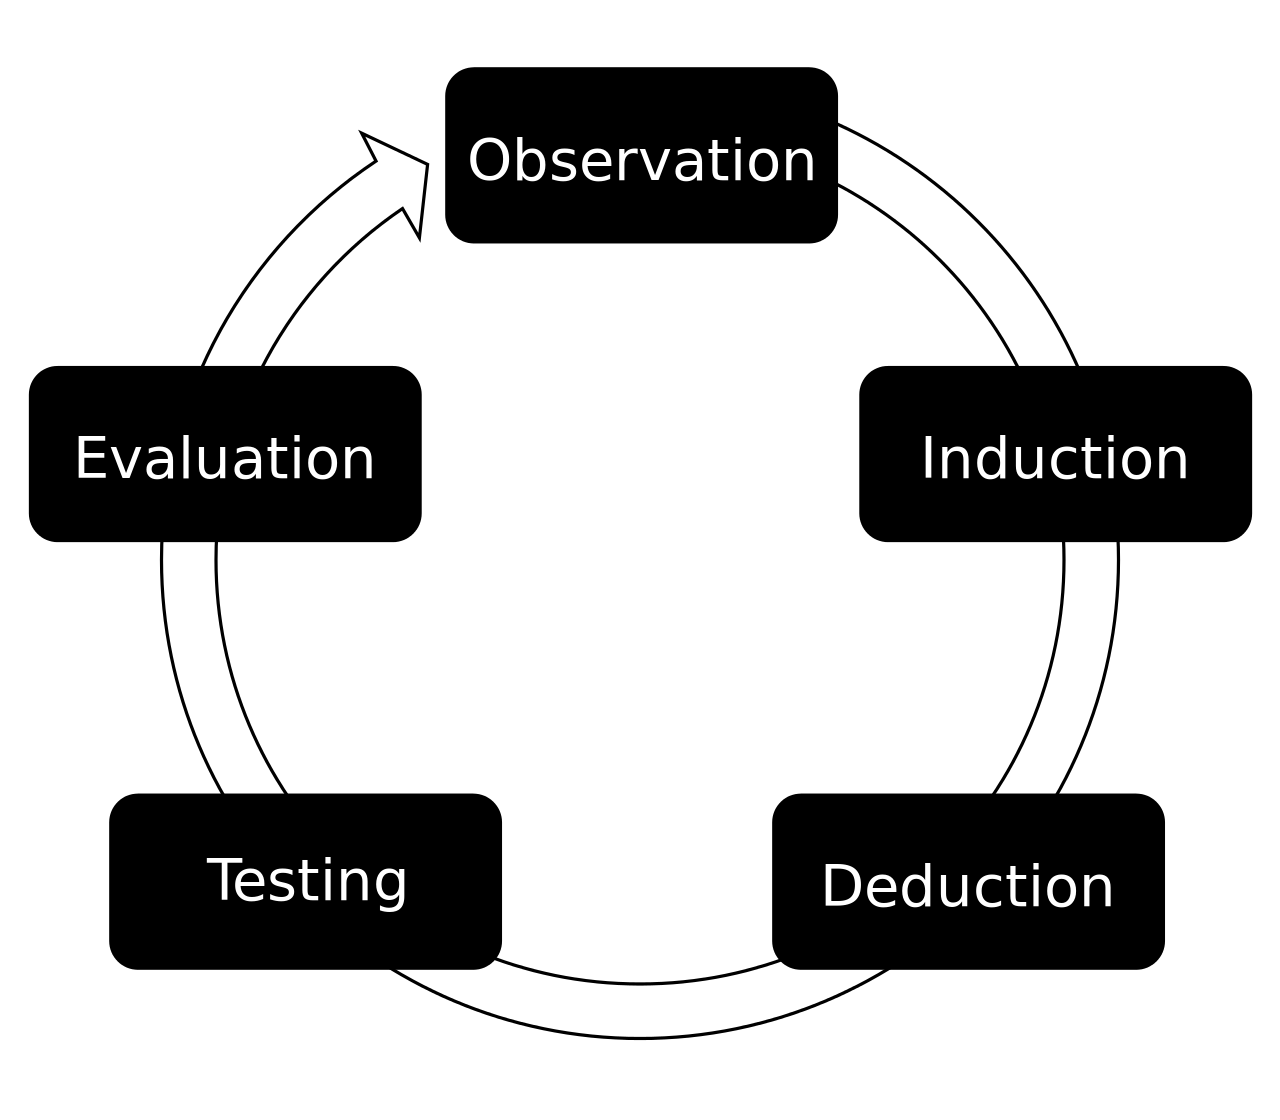
\includegraphics[width=0.45\textwidth]{Figuras/MetodologiaEmpirica.png}}
    \caption{Ciclo empírico de A.D. de Groot (Fuente: Wikipedia\autocite{InvestigacionEmpirica2020})} 
    \label{fig:CicloEmpirico}
\end{figure}
\section{Metodología de desarrollo}

El modelo en espiral (Fig.\ref{fig:MetodologiaEspiral}) formará parte del ya mencionado Ciclo empírico y agrupará los pasos de formulación de los experimentos y su ejecución. Se ha optado por incluir esta metodología dentro de otra para detallar más profundamente cómo será el proceso de desarrollo de software derivado de la investigación realizada.
\\ \\
Se ha elegido este modelo entre otros por varias razones importantes:
\begin{itemize}
    \item Define claramente lo que es un ciclo completo, los pasos a dar y las tareas a realizar. También fija los objetivos al inicio de cada ciclo de la espiral, lo que unido al paso de inducción del ciclo empírico implica que se definen objetivos claros y concisos sobre las hipótesis planteadas.
    \item Al ser un modelo continuo, se pueden realizar tantas iteraciones sobre la espiral como se necesiten, permitiendo desarrollar tantos experimentos como hipótesis se plantean en el apartado de inducción del ciclo empírico. Además, cada vuelta de la espiral incluye el desarrollo de prototipos (lo que en este caso sería un experimento), que al contar con una fase de integración consigue que puedan coexistir todos en el mismo entorno de desarrollo.
    \item Cumple con las fases de Deducción y Testeo del ciclo empírico ya que incluye los pasos de estas en la fase de desarrollo de la espiral.
    \item Por último y más importante, se ha elegido esta metodología porque tiene en cuenta la gestión y análisis de riesgos. Esto tiene gran importancia al tratarse de un proyecto complejo con múltiples dispositivos y tanta cantidad de pruebas a realizar.
\end{itemize}

\begin{figure}[thbp]
    \centering
    \fbox{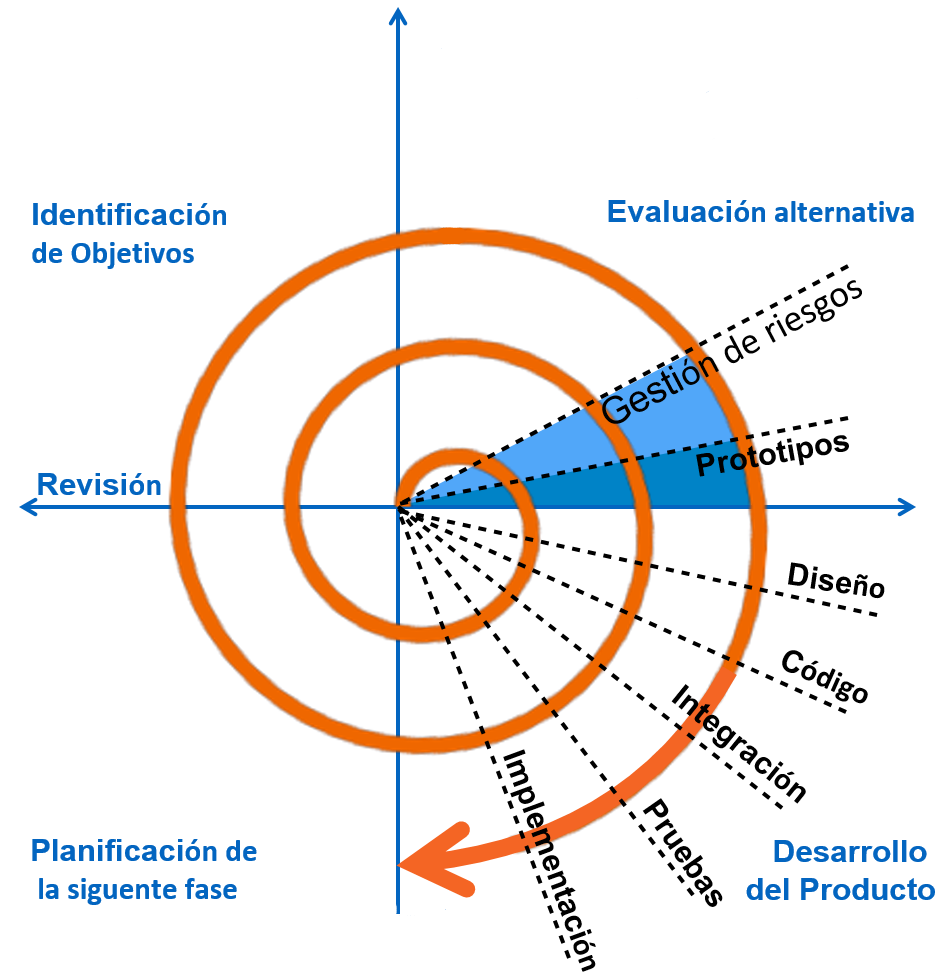
\includegraphics[width=0.6\textwidth]{Figuras/MetodologiaEspiral.png}}
    \caption{Modelo en el Espiral, Autor Desconocido (Fuente: Blog\autocite{CicloVidaSoftware2016})} 
    \label{fig:MetodologiaEspiral}
\end{figure}

\section{Conclusión}
Partiendo del ciclo empírico, escisión de la metodología de investigación cuantitativa, se hará especial incapié en la continua reflexión y teorización sobre el modelo de fededrated learning implantado. 
\\ \\
Para el correcto desarrollo del software, las anteriormente mencionadas fases de deducción y testeo serán incluidas en el modelo de la espiral, consiguiendo así, una gestión eficiente y precisa sobre los pasos a dar tanto en investigación como en el desarrollo de software.
\\ \\
Como se ha comentado anteriormente, la agrupación de estas dos metodologías permitirá combinar la investigación con el desarrollo de software, descubriendo a base de prueba y error y a base de analizar los resultados las mejores soluciones para el sistema de recomendación basado en federated learning.
\\ \\
Por lo cual, una vez el alumno haya definido claramente el problema, su alcance y se haya formado en la tecnología, podrá comenzar a utilizar el ciclo presente en la figura \ref{fig:MetodologiaCombinada}.

\begin{figure}[thbp]
    \centering
    \fbox{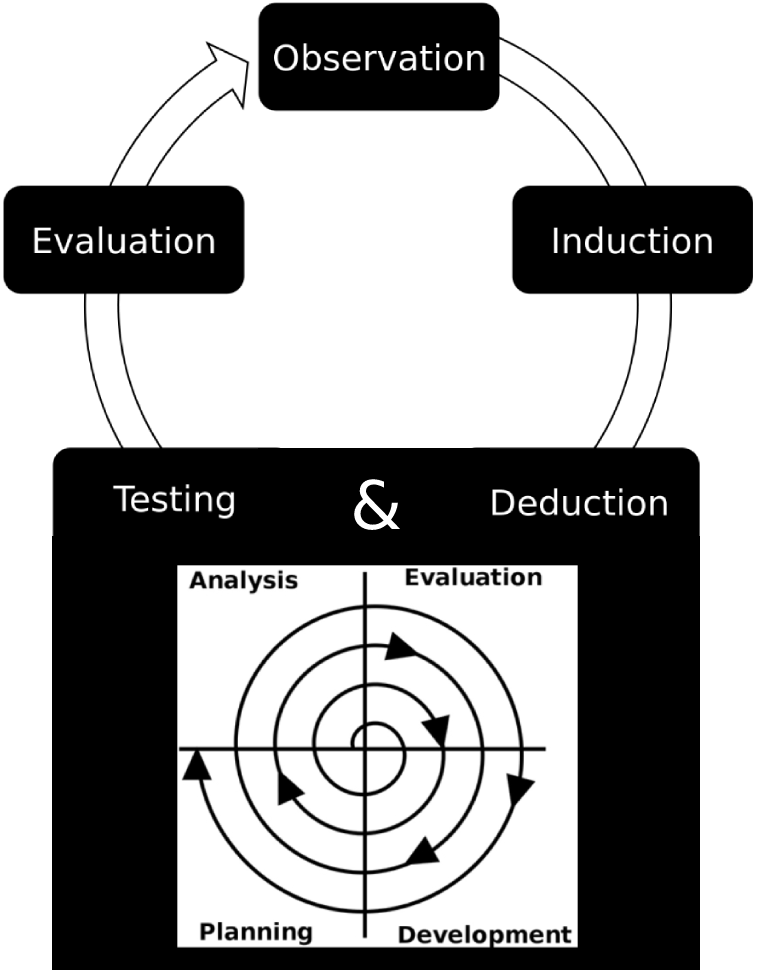
\includegraphics[width=0.6\textwidth]{Figuras/MetodologiaCombinada.png}}
    \caption{Metodología de trabajo del proyecto final de grado (Autor: Ibai Guillén)} 
    \label{fig:MetodologiaCombinada}
\end{figure}
\fancyhead[LE]{}
\newpage
\thispagestyle{plain}
\cleardoublepage

%\chapter{Sistema de recomendación}
\thispagestyle{fancy}
\section{LightFM}
LightFM es una implementación en python de varios algotitmos populares de recomendación.
\subsection{Creación del modelo}
El paso de creación del modelo es un paso complejo puesto que conlleva la correcta gestión de muchos datos e información. Asimismo, estos datos han de estar correctamente estructurados y construidos, puesto que LightFM requiere que la información este convertida a matrices dispersas y no tolera elementos vacíos en ellas. Para ello LightFM proveé de herramientas de creación de datasets que facilitan la creación de las matrices, de forma que sea más fácil incluirlas en el modelo. 
\\ \\
Entre estas erramientas se encuentran:

\begin{itemize}
    \item \textit{build\_user\_features($\ldots$)} \quad Permite crear la matriz CSR de usuarios y atributos de usuarios.
    \item \textit{build\_item\_features($\ldots$)} \quad Permite crear la matriz CSR  de items y atributos de items.
    \item \textit{build\_interactions($\ldots$)} \quad Permite crear las matriz COO de interacciones y las matriz COO de sus correspondientes pesos.
\end{itemize}

Hay que tener en cuenta que las matrices CSR (Compressed Sparse Row) hacen referencia a las matrices que admiten operaciones matriciales y acceso eficientemente; y que las matrices COO (Coordinate list) hacen referencia a las matrices que soportan modificaciones eficientemente, son generalmente utilizadas para construir matrices.


\subsubsection{Atributos de los usuario}
Para crear el modelo es necesario, entre otras cosas, disponer de las características de los usuarios. En este caso contamos con multitud de atributos sobre cada usuario: edad, género, nivel educativo, país, cultura de trabajo, perfil PST (Pinball, Shortcut, Thought-ful), barreras, intenciones y confianza.
\\ \\
Para convertir toda esa información del usuario a la matriz CSR que exige LightFM habrá que llamar a \textit{build\_user\_features($\ldots$)} con los IDs de usuario y y sus atributos, formando una lista que tenga listas de los IDs de los usuarios con sus listas de atributos, es decir:
\begin{align*}
    \begin{bmatrix}
        \begin{bmatrix} 
            userId$$_{1}$$ & \begin{bmatrix} feature$$_{11}$$ &\cdots & feature$$_{1w}$$ \end{bmatrix}$$_1$$
        \end{bmatrix}
        &
        \ldots
        &
        \begin{bmatrix} 
            userId$$_{v}$$ & \begin{bmatrix} feature$$_{v1}$$ &\cdots & feature$$_{vw}$$ \end{bmatrix}$$_v$$
        \end{bmatrix}
    \end{bmatrix}
\end{align*}
Teniendo en cuenta que:
\begin{align*}
    \textit{v}\gets & \textit{Cantidad de IDs de usuario }
    &&\\
    \textit{w} \gets & \textit{Contidad de atributos por usuario}
    &&\\
    \textit{userId$_{v}$} \gets & \textit{ID del usuario v}
    &&\\
    \textit{feature$_{vw}$} \gets & \textit{Atributo w del usuario v}
\end{align*}
%
Una vez creada la lista y pasado como parámetro al método, obtendremos la matriz CSR de atributos de usuario.

\subsubsection{Atributos de los elementos}
Además de los usuarios y de sus atributos, también se ha de disponer de los elementos a ordenar en el ranking, llamados items, y de sus características. En este caso estos items representan las estrategias de persuasión por las que se preguntó a los usuarios en el cuestionario. Sin embargo, al contrario que en el punto anterior, no contamos con tantos atributos sobre estos items, sino que cada estrategia de persuasión cuenta con dos atributos llamados dimensiones. Estos atributos no se encuentran presente en todas las estrategias, lo que da como resultado que haya algunas que tengan dos, una o ninguna dimension.
\\ \\
Para convertir toda esa información de los items a la matriz CSR que exige LightFM habrá que llamar a \textit{build\_item\_features($\ldots$)} con los IDs de las estrategias y y sus atributos, formando una lista que tenga listas de los IDs de las estrategias con sus listas de atributos, es decir:
\begin{align*}
    \begin{bmatrix}
        \begin{bmatrix} 
            itemId$$_{1}$$ & \begin{bmatrix} feature$$_{11}$$ &\cdots & feature$$_{1w}$$ \end{bmatrix}$$_1$$
        \end{bmatrix}
        &
        \ldots
        &
        \begin{bmatrix} 
            itemId$$_{v}$$ & \begin{bmatrix} feature$$_{v1}$$ &\cdots & feature$$_{vw}$$ \end{bmatrix}$$_v$$
        \end{bmatrix}
    \end{bmatrix}
\end{align*}
Teniendo en cuenta que:
\begin{align*}
    \textit{v}\gets & \textit{Cantidad de IDs de estrategias }
    &&\\
    \textit{w} \gets & \textit{Contidad de dimensiones por estrategia}
    &&\\
    \textit{itemId$_{v}$} \gets & \textit{ID de la estrategia v}
    &&\\
    \textit{feature$_{vw}$} \gets & \textit{Atributo w de la estrategia v}
\end{align*}
%
Una vez creada la lista y pasado como parámetro al método, obtendremos la matriz CSR de atributos de usuario.
%
%
\subsubsection{Interacciones}


Para crear un modelo de LightFM se necesita

user\_features, item\_features 

model = LightFM() 

% model.fit(train\_interactions,
%         user\_features=user\_features,
%         sample\_weight=train\_weights,
%         epochs=100,
%         num\_threads=4,
%         verbose=False)
% ranks\_test = model.predict\_rank(test\_interactions, 
%         #train\_interactions= train\_interactions, 
%         user\_features=user\_features,
%         check\_intersections=True)                    

\subsection{Ajuste}
\subsection{Predicción}


\section{Evaluación}
La evaluación de los resultados obtenidos de las predicciones de los modelos es un apartado fundamental que permite analizar la eficacia de estas predicciones. Además, la utilización de métricas y técnicas permitirá poder comparar los resultados entre sí para poder demostrar si la predicción es correcta, aceptable o erronea.
\subsection{Métricas}

Antes de realizar el ranking hay que definir una métrica que permita evaluar la precisión de este, y por ende, la precisión del modelo. Para esta labor se ha utilizado la métrica NDPM, medida de rendimiento normalizada basada en la distancia. Esta métrica se utiliza para sistemas de recomendación basados en ranking y mide la eficacia del modelo para predecir el correcto orden de los n elementos del ranking. 
%
\begin{align*}
    \textit{NDPM} && \parbox[t]{8cm}{\raggedright Medida de rendimiento normalizada basada en la distancia (Normalized Distance-based Performance Measure)} \nonumber 
\end{align*}
%
Cuanto menor sea el NDPM, mayor será la similitud entre el ranking predicho por el modelo y entre el declarado por el usuario. En el caso ideal donde la predicción hubiera acertado por completo el ranking del usuario, el NDPM sería 0. En caso contrario, es decir, que hubiera predicho un orden totalmente erroneo, el NDPM sería 1.

\subsection{Técnicas}

La lista de elementos a ser ordenados por los modelos LightFM son los siguientes:
\begin{alignat*}{1}
strats = \begin{bmatrix} 'v2' & 'v5' & 'v6' & 'v7' & 'v10' & 'v11' & 'v15' & 'v17' & 'v19' & 'v20' \end{bmatrix} 
& \\
\parbox[t]{8cm}{\raggedright Lista de estrategias a clasificar del 1 a n} \nonumber
\end{alignat*}
En esta lista solo aparecen los elementos más relevantes de las encuestas, ya que (nidea)
%%

\begin{align*}
%%
i && \parbox[t]{8cm}{\raggedright Número de modelos LightFM} \nonumber 
%%
&& \\
%%
n && \parbox[t]{8cm}{\raggedright Número de elementos a incluir en el ranking} \nonumber 
%%
&& \\
%%
m && \parbox[t]{8cm}{\raggedright Número de epochs sobre cada dataset} \nonumber
%%
&& \\
%%
a_{mn} && \parbox[t]{8cm}{\raggedright Índice del elemento n de la lista de strats en el ranking calculado en la epoch m} \nonumber
%%
&& \\
%%
matriz_{i[m,n]}= \begin{pmatrix}
 a_{11}  &  a_{12}  &  \cdots   & a_{1n} \\ 
 a_{21}  &  a_{22}  &  \cdots   & a_{2n}\\ 
 \vdots  &  \vdots  &  \ddots & \vdots  \\ 
 a_{m1}  &  a_{m2}  &  \cdots   & a_{mn}
\end{pmatrix}  && \parbox[t]{8cm}{\raggedright Matriz numpy de los resultados de la predicción del modelo i} \nonumber
%%
&& \\ \\
%%
prediction_{m[1,n]}= \begin{bmatrix} a_{1}  &  a_{2}  &  \cdots   & a_{n} \end{bmatrix} && \parbox[t]{8cm}{\raggedright Lista de los índices de los n strat para el ranking del epoch m} \nonumber
%%
\\ \\
Predictions_{i[m,n]} = \begin{bmatrix}
 \begin{bmatrix} a_{11}  &  a_{12}  &  \cdots   & a_{1n} \end{bmatrix} \\ 
 \begin{bmatrix} a_{21}  &  a_{22}  &  \cdots   & a_{2n} \end{bmatrix}\\ 
 \vdots \\ 
 \begin{bmatrix} a_{m1}  &  a_{m2}  &  \cdots   & a_{mn} \end{bmatrix}
\end{bmatrix} && \parbox[t]{8cm}{\raggedright Lista de predicciones del modelo i por cada epoch m} \nonumber
%%
&& \\ \\
%%
ndpms_{i[1,m]}= \begin{bmatrix} ndpm_{1}  &  ndpm_{2}  &  \cdots   & ndpm_{m} \end{bmatrix} && \parbox[t]{8cm}{\raggedright Lista de NDPMs calculados sobre las predicciones de cada epoch m del  modelo i LightFM} \nonumber
\end{align*}
\\ \\
%%
Si se desagrupan las predicciones realizadas por cada epoch m y se agrupan en función de cada strat n tendremos la lista de valores que el modelo i da a cada uno de los elementos n de la lista de los strat. Esto quiere decir que si se agrupan en función del elemento que se ordena en el ranking en vez de en por predicción se obtendrá la lista de todas las predicciones de posición para cada uno de los elementos a ordenar.
\begin{alignat*}{1}
\parbox[t]{8cm}{\raggedright }\nonumber & \\
Predictions_{i[m,n]}= \begin{bmatrix}
\begin{bmatrix} a_{11} \\ a_{21} \\ \vdots \\ a_{m1} \end{bmatrix} 
& \begin{bmatrix} a_{12} \\ a_{22} \\ \vdots \\ a_{m2} \end{bmatrix} 
& \cdots
& \begin{bmatrix} a_{1n} \\ a_{2n} \\ \vdots \\ a_{mn} \end{bmatrix} 
\end{bmatrix}
\end{alignat*}
Una vez teniendo la lista de los valores para cada elemento se pueden aplicar métodos estadísticos como la media(\(\bar{x}\)), mediana(\(\tilde{x}\)) o moda (\(\hat{x}\)) para crear una única predicción consensuada para el modelo i al que pertenecen estas predicciones. Esta predicción consensuada permitirá combinar los rankings generados durante cada epoch para poder obtener la máxima precisión posible y la mínima desviación típica.
\begin{alignat*}{2}
\bar{x}   &  \parbox[t]{8cm}{\raggedright Media} \nonumber \\
\tilde{x} & \parbox[t]{8cm}{\raggedright Mediana} \nonumber \\
\hat{x}   & \parbox[t]{8cm}{\raggedright Moda} \nonumber
\end{alignat*}
Consenso por media de las m predicciones para el modelo i:
\begin{alignat*}{1}
\overline{consensous_{i[1,m]}}= \begin{bmatrix} \overline{a_{11}} &  \overline{a_{21}}  &  \cdots   & \overline{a_{m1}} \end{bmatrix} 
\end{alignat*}
\\
Consenso por mediana de las m predicciones para el modelo i:
\begin{alignat*}{1}
\widetilde{consensous_{i[1,m]}}= \begin{bmatrix} \widetilde{a_{11}} &  \widetilde{a_{21}}  &  \cdots   & \widetilde{a_{m1}} \end{bmatrix} 
\end{alignat*}
\\
Consenso por moda de las m predicciones para el modelo i:
\begin{alignat*}{1}
\widehat{consensous_{i[1,m]}}= \begin{bmatrix} \widehat{a_{11}} &  \widehat{a_{21}}  &  \cdots   & \widehat{a_{m1}} \end{bmatrix} 
\end{alignat*}
%%
\\ \\ \\
%%

\begin{algorithm}
\caption{Entrenamiento del modelo}\label{euclid}
\begin{algorithmic}[1]
\Procedure{Experimento}{}
\State $\textit{// Lista de estrategias a clasificar del 1 a n:}$
\State $strats \gets \begin{bmatrix} 'v2' & 'v5' & 'v6' & 'v7' & 'v10' & 'v11' & 'v15' & 'v17' & 'v19' & 'v20' \end{bmatrix}$ 
\\
\State $i \gets \parbox[t]{8cm}{\raggedright \textit{Cantidad de modelos a crear.}}\nonumber$
\State $m \gets \parbox[t]{8cm}{\raggedright \textit{Cantidad de epochs sobre cada modelo i.}}\nonumber$
\\
\State $\textit{// Lista de listas de NDPMs, de cada predicción de la epoch m, de cada modelo i:}$
\State \textit{// $[[ndpm_{1}$, $ndpm_{2}$, \ldots, $ndpm_{m}]_{1}$, \ldots, $[ndpm_{1}$, $ndpm_{2}$, \ldots, $ndpm_{m}]_{i}]$ } 
\State $\textit{ndpms} \gets [[\textit{float}_{m}]_{i}]$
\\
\State $\textit{// Lista de NDPMs, de cada predicción consensuada, de cada modelo i:}$
\State \textit{// $[ndpm_{1}$, $ndpm_{2}$, \ldots, $ndpm_{i}]$} 
\State $\textit{commonNdpms} \gets [\textit{float}_{i}]$
\\
\State \textit{// Lista de los índices de los n strat para el ranking del epoch m}
\State $\textit{// } 
\begin{bmatrix} float_{n} \end{bmatrix} 
=
\begin{bmatrix} a_{1}  &  a_{2}  &  \cdots   & a_{n} \end{bmatrix}$
%
\State \textit{// Lista de los índices de los n strat, de cada epoch m}
\State $ \textit{// }
\begin{bmatrix} \begin{bmatrix} float_{n} \end{bmatrix}_{m} \end{bmatrix}
=
\begin{bmatrix} 
    \begin{bmatrix} 
        $$a_{1}$$ & $$a_{2}$$ & \ldots & $$a_{n}$$ 
    \end{bmatrix}$$_{1}$$ 
    & \ldots 
    & \begin{bmatrix} 
        $$a_{1}$$ & $$a_{2}$$ & \ldots & $$a_{n}$$ 
    \end{bmatrix}$$_{m}$$
\end{bmatrix}  $
%
\State \textit{// Lista de los índices de los n strat, de cada epoch m, de cada modelo i}
\State $\textit{// }
\begin{bmatrix} \begin{bmatrix} \begin{bmatrix} float_{n} \end{bmatrix}_{m} \end{bmatrix}_{i} \end{bmatrix}
=
\begin{bmatrix}
    \begin{bmatrix}
        \begin{bmatrix} $$a_{1}$$  &  $$a_{2}$$  &  \cdots   & $$a_{n}$$ \end{bmatrix}_{1} \\ 
        \vdots \\ 
        \begin{bmatrix} $$a_{1}$$  &  $$a_{2}$$  &  \cdots   & $$a_{n}$$ \end{bmatrix}_{m}
    \end{bmatrix}_{1}
    &
    \cdots
    &
    \begin{bmatrix}
        \begin{bmatrix} $$a_{1}$$  &  $$a_{2}$$  &  \cdots   & $$a_{n}$$ \end{bmatrix}_{1} \\ 
        \vdots \\ 
        \begin{bmatrix} $$a_{1}$$  &  $$a_{2}$$  &  \cdots   & $$a_{n}$$ \end{bmatrix}_{m}
    \end{bmatrix}_{i}
\end{bmatrix}$
\\
\State $\textit{predictions} \gets \begin{bmatrix} \begin{bmatrix} \begin{bmatrix} float_{n} \end{bmatrix}_{m} \end{bmatrix}_{i} \end{bmatrix}$
\BState \emph{loop}:
\For {$\textit{int}(j) \gets 0$ \textbf{to} $\textit{range}(i)$}
    \State $userFeatures, itemFeatures \gets features()$ $\parbox[t]{4cm}{//\raggedright \textit{Obtiene todas las características de los usuarios y de los items}}\nonumber$
    \\
    \State $trainInteractions \gets \parbox[t]{8cm}{\raggedright \textit{Interacciones para entrenar el modelo. }}\nonumber$
    \State $testInteractions \gets \parbox[t]{8cm}{\raggedright \textit{Interacciones para probar el modelo. }}\nonumber$
    \\
    \State $trainWeights \gets \parbox[t]{8cm}{\raggedright \textit{Peso de las interacciones de entrenamiento. }}\nonumber$
    \\
    \State $trainUerid \gets \parbox[t]{8cm}{\raggedright \textit{IDs de los usuarios que se utilizan para entrenar. }}\nonumber$
    \State $testUserid \gets \parbox[t]{8cm}{\raggedright \textit{IDs de los usuarios que se utilizan para probar. }}\nonumber$
    \BState \emph{loop}:
    \For {$\textit{int}(k) \gets 0$ \textbf{to} $\textit{range}(m)$}
        \State $modelo \gets LightFM()$ $\parbox[t]{8cm}{//\raggedright \textit{Se crea el modelo LightFM }}\nonumber$
        \\
        \State$\textit{//Ajustar modelo a la información extraida:}$
        \State $modelo.fit(trainInteractions,userFeatures ,trainWeights)$ 
        \\
        \State$\textit{//Predicción del modelo para las interacciones de prueba:}$
        \State $predictRank \gets modelo.predict(testInteractions, userFeatures)$
        \\
        \State $ndpms[i].append(ndpm(ranks_test))$ $\parbox[t]{8cm}{//\raggedright \textit{Añadir el valor NDPM del ranking creado por el modelo i, en la epoch m, a la lista de NDPMs del modelo i}}\nonumber$

        %predictions[i].append(ranks_test.data)

        \State \textbf{close};
    \EndFor
    
    \State $i \gets i-1$.
    \State \textbf{goto} \emph{loop}.
    \State \textbf{close};
\EndFor
%%
%%
\EndProcedure
\algstore{Experimento}
\end{algorithmic}
\end{algorithm}
%%
\begin{algorithm}
\begin{algorithmic}[1]
\algrestore{Experimento}
\BState \emph{top}:
\If {$i > \textit{stringlen}$} \Return false
\EndIf
\State $j \gets \textit{patlen}$
\BState \emph{loop}:
\If {$\textit{string}(i) = \textit{path}(j)$}
\State $j \gets j-1$.
\State $i \gets i-1$.
\State \textbf{goto} \emph{loop}.
\State \textbf{close};
\EndIf
\State $i \gets i+\max(\textit{delta}_1(\textit{string}(i)),\textit{delta}_2(j))$.
\State \textbf{goto} \emph{top}.
\end{algorithmic}
\end{algorithm}
%%
\begin{algorithm}
\caption{Algoritmo de consenso}\label{euclid}
\begin{algorithmic}[1]
\Procedure{Consensuar}{matriz}
\State a

\State $\textit{stringlen} \gets \text{length of }\textit{string}$
\State $i \gets \textit{patlen}$

\BState \emph{top}:
\If {$i > \textit{stringlen}$} \Return false
\EndIf
\State $j \gets \textit{patlen}$
\BState \emph{loop}:
\If {$\textit{string}(i) = \textit{path}(j)$}
\State $j \gets j-1$.
\State $i \gets i-1$.
\State \textbf{goto} \emph{loop}.
\State \textbf{close};
\EndIf
\State $i \gets i+\max(\textit{delta}_1(\textit{string}(i)),\textit{delta}_2(j))$.
\State \textbf{goto} \emph{top}.
\EndProcedure
\end{algorithmic}
\end{algorithm}




%\cleardoublepage

\printbibliography

%Nueva página en blanco total 
%\newpage
%\thispagestyle{empty}
%Evitamos crear doble pagina y obligamos a empezar en página impar
%\cleardoublepage
%%\appendixname %nombre del capitulo como índice
\chapter{Protección de Datos en la Unión Europea y España}\label{appendix:ProteccionDatos}
\thispagestyle{fancy}
\fancyhead[LE]{Apéndice \thechapter.Protección de Datos en la Unión Europea y España} 
\begin{refsection}

\section{Preludio}
Ante la llegada de las Tecnologías de la Información y la Comunicación (TIC), la Organización para la Cooperación y el Desarrollo Económicos (OCDE) decidió definir unas directrices el 23 de septiembre de 1980 que regulen \textit{".. la protección de la privacidad y el flujo transfronterizo de datos personales ... "} \autocite[\ppno 1]{oecdOECDGuidelinesProtection2002}. Este fue uno de los primeros intentos de regular la gestión y utilización de los datos personales.
\\ \\
No llegaron medidas concretas a Europa hasta el 24 de octubre de 1995, cuando el Parlamento Europeo y el Consejo Europeo publicaron la \textit{"Directiva 95/46/CE"} \autocite{DIRECTIVA9546} con el objetivo de crear un marco jurídico que garantizase la protección de los datos y la libre circulación de estos\footnote{Las directivas de la UE no son legalmente vinculantes para los ciudadanos, se dirigen a todos los estados miembros y cada uno deberá transponer la directiva a las leyes locales}. Por eso, en España se creó la \textit{"Ley Orgánica 15/1999, de 13 de diciembre, de Protección de Datos de Carácter Personal"} \autocite{LEYORGANICA15} más conocida por sus siglas LOPD, que era la encargada de garantizar el cumplimiento de la directiva europea en España. 
\\ \\
Ante la ausencia de leyes que garantizaran el cumplimiento de los derechos humanos en internet, algunos autores empezaron a definir los derechos digitales. Una de las primeras declaraciones de derechos fundamentales tecnológicos fue la de Robert B. Gelman, que en 1997 difundió una propuesta de \textit{"Declaración de los Derechos Humanos en el Ciberespacio"}, basada en la Declaración Universal de los Derechos Humanos de 1948.
\\ \\
Sin embargo, aunque el trabajo de Robert B. Gelman fue ampliamente apoyado por una gran comunidad de expertos, no ha sido hasta la entrada en el siglo XXI (cuando las TIC ya han conseguido una gran relevancia en la sociedad) que se ha empezado a atisbar la necesidad de derechos digitales inherentes de vivir en una sociedad tecnológica. Tanto es así, que varios autores empezaron a escribir sobre la necesidad de una nueva generación de derechos humanos que incluyese el campo de la tecnología.
\\ \\
La corriente pro derechos digitales llegó inclusive a la Unión Europea, que en el año 2000 redactó la \textit{"Carta de los Derechos Fundamentales de la Unión Europea"} \autocite{CartaDerechosFundamentalesb} en Niza con el objetivo de \textit{"... reforzar la protección de los derechos fundamentales a tenor de la evolución de la sociedad, del progreso social y de los avances científicos y tecnológicos."} \autocite[\ppno 5]{CartaDerechosFundamentalesb}. El problema es que no pasó a ser jurídicamente vinculante hasta el año 2009 junto con el Tratado de Lisboa. Esta carta es especialmente innovadora en cuanto a la protección de datos de carácter personal, puesto que establecía como derecho fundamental la protección de estos en el artículo 8. En este artículo se establecía que además, estos se tratarían de modo leal y con el consentimiento de la persona afectada. Asimismo, la persona afectada tendría derecho a acceder a los datos recogidos, así como a la rectificación de los mismos.

\section{Legislación}\label{appendix:ProteccionDatos_Legislacion}
La legislación vigente en Europa cambió radicalmente en el 2016, el parlamento europeo adoptó nuevas medidas para la era digital.
\\ \\
El 5 de mayo de 2016 entró en vigor la Directiva (UE) 2016/680 \autocite{DIRECTIVAUE2016}, reconocida como la Directiva sobre protección de datos en el ámbito penal, \textit{"... relativa a la protección de las personas físicas en lo que respecta al tratamiento de datos personales por parte de las autoridades competentes para fines de prevención, investigación, detección o enjuiciamiento de infracciones penales o de ejecución de sanciones penales, y a la libre circulación de dichos datos ..."} \autocite[\ppno 1]{DIRECTIVAUE2016}. La Comisión Europea define esta medida en su página web \autocite{ProteccionDatosUEa} como:

\begin{minipage}[t]{0.2\linewidth}
\end{minipage}
\hfill
\begin{minipage}[t]{0.9\linewidth}
  \textit{"... protege el derecho fundamental de los ciudadanos a la protección de sus datos cuando los utilicen las autoridades policiales y judiciales a efectos de aplicación de la ley. Más concretamente, la Directiva garantizará que se protejan adecuadamente los datos personales de víctimas, testigos y sospechosos de delitos, además de facilitar la cooperación transfronteriza en la lucha contra la delincuencia y el terrorismo."}
\end{minipage}
\\ \\ \\
El 24 de mayo de 2016 el Reglamento (UE) 2016/679 \autocite{REGLAMENTOUE2016}, reconocido como el Reglamento General de Protección de Datos (RGPD). \textit{"... relativo a la protección de las personas físicas en lo que respecta al tratamiento de datos personales y a la libre circulación de estos datos …"} \autocite[\ppno 2]{REGLAMENTOUE2016}. La Comisión Europea define esta medida en su página web como:

\begin{minipage}[t]{0.2\linewidth}
\end{minipage}
\hfill
\begin{minipage}[t]{0.9\linewidth}
  \textit{"... es una medida esencial para fortalecer los derechos fundamentales de las personas en la era digital y facilitar la actividad económica, ya que aclara las normas aplicables a las empresas y los organismos públicos en el mercado único digital. Además, la existencia de una norma única pone fin a la fragmentación en distintos sistemas nacionales y a las cargas administrativas innecesarias."}
\end{minipage}
\\ \\ \\
Esta legislación no sería aplicable hasta dos años más tarde, el 6 y 25 de mayo de 2018 respectivamente. Dos años durante los cuales cualquier empresa de la unión o cualquier empresa que tenga negocios en la Unión Europea se debía adaptar a la nueva normativa.
\\ \\
El objetivo principal de este reglamento era proteger a las personas físicas en cuanto al tratamiento de sus datos personales y a la libre circulación de estos. Estos datos son de naturaleza sensible, puesto que pueden revelar la identidad de la persona, ya sea mediante el nombre completo, la dirección de su domicilio, el número de tarjeta bancaria, etc.
\\ \\
Entre las cuestiones más relevantes del RGPD destacan: 
\begin{itemize}
  \item La transparencia: obliga a las organizaciones a comunicar a los usuarios el tratamiento que se realiza a sus datos.
  \item El derecho a la rectificación y borrado: cada usuario tendrá derecho a pedir que se rectifiquen sus datos en caso de ser inexactos. Además, los usuarios tendrán derecho a que las organizaciones borren sus datos y rescindir el consentimiento de tratamiento de ellos.
  \item Derechos sobre el procesamiento: cada usuario podrá solicitar la limitación de procesamiento de sus datos, así como negarse a que se usen en tomas de decisiones o en perfiles automatizados, aparte, también podrá solicitar que le entreguen sus datos en formato estructurado cuando sea posible.
\end{itemize}
La directiva sobre protección de datos en el ámbito penal y el RGPD dejaron obsoleta la LOPD española, por lo cual, para adaptarse al nuevo marco jurídico europeo el 7 de diciembre de 2018 entró en vigor la \textit{"Ley Orgánica 3/2018, de 5 de diciembre, de Protección de Datos Personales y Garantía de los Derechos Digitales"} \cite{samperLeyOrganica20182020} (LOPD-GDD), acorde con el RGPD.
\\ \\
Esta ley transpone el RGPD europeo a la legislación española, incluyendo medidas como:
\begin{itemize}
  \item La incorporación del término privacidad desde el diseño, lo que quiere decir que deben elaborarse procesos empresariales teniendo en cuenta la LOPD-GDD desde un primer momento. 
  \item El consentimiento, donde se obliga a las organizaciones a obtener el consentimiento explícito para el tratamiento de datos de las personas, estas personas, además, podrán solicitar la portabilidad de sus datos o la eliminación de los mismos.
\end{itemize}
Sin embargo, la LOPD-GDD no se ciñe únicamente a adaptar el RGPD a la legislación Española, fue la primera ley europea de protección de datos en incluir explícitamente los derechos digitales de las personas en los entornos digitales.

\section{Derechos fundamentales}\label{appendix:ProteccionDatos_Derechos}

Como se ha comentado en el apartado anterior, con la entrada en vigor de la LOPD-GDD España se convirtió en el primer país europeo en garantizar los derechos digitales. Estos derechos digitales llegaron en 2018 en el Título X de la LOPD-GDD, titulado \textit{"Garantía de los derechos digitales"}, en respuesta a la Carta de los Derechos Fundamentales de la Unión Europea y a las nuevas medidas del Reglamento (UE) 2016/679 y de la Directiva (UE) 2016/680. 
\\ \\
Varios de los derechos recogidos en la LOPD-GDD fueron:
\begin{itemize}
  \item El derecho a la intimidad y uso de dispositivos digitales en el ámbito laboral.
  \item El derecho a la desconexión digital en el ámbito laboral.
  \item Derecho al olvido en búsquedas de Internet.
  \item El derecho al testamento digital.
\end{itemize}
Este paso adelante por parte del estado español incentivó a que un año después de la entrada en vigor de la LOPD-GDD, el Ilustre Colegio de la Abogacía de Barcelona (ICAB) presentase la \textit{"Carta de Barcelona por los Derechos de la Ciudadanía en la Era Digital"} \autocite{CartaBarcelonaPor}, apoyada por universidades y entidades de la sociedad civil. 
\\ \\
A la vista de la relevancia e impacto del tema, el gobierno español (representado por el Ministerio de Asuntos Económicos y Transformación Digital), se inspirará en la carta del ICAB para redactar la pionera \textit{"Carta de Derechos Digitales"} \autocite{CartaDerechosDigitales} de España, que contribuirá con los objetivos ya avanzados en el Título X de la LOPD-GDD. Se prevé que sea aprobada antes de 2022 para la estrategia España Digital 2025.
\\ \\
Esta carta cuenta con 25 puntos de alta relevancia entre los que están los recogidos en el anteriormente mencionado Título X de la LOPD-GDD, y entre otros, algunos de especial impacto en el desarrollo de este proyecto: los derechos ante la Inteligencia Artificial (Derecho XXIII) y el derecho a no ser localizado y perfilado (Derecho V). 
\\ \\
El derecho a no ser localizado y perfilado deja claro que cada persona tiene derecho a la \textit{"... libre autodeterminación individual (...) a no ser objeto de localización, ni a ser sometido a análisis de la personalidad o conducta que impliquen el perfilado de la persona"}, además, añade que sólo se podrán realizar \textit{"... tratamientos de información personal con el consentimiento de la persona afectada ..."}.
\\ \\
En cuanto al derecho ante la Inteligencia Artificial expone como primer punto que, en lo que concierne al desarrollo y ciclo de vida de esta, \textit{"Se deberá garantizar el derecho a la no discriminación algorítmica …"}. Además. en procesos de decisión automatizada las personas tienen derecho a \textit{"Solicitar una supervisión e intervención humana"} o \textit{"Impugnar las decisiones automatizadas o algorítmicas"}.
\\ \\
La carta, al no estar aprobada aún, no es legalmente vinculante, por lo que no es de obligado cumplimiento. Sin embargo, deja clara la orientación que van a tomar los derechos digitales en los próximos años.

\newpage
\thispagestyle{empty}
\cleardoublepage
\printbibliography[heading=subbibliography]

\end{refsection}


\end{document}
%Función de final de documento.

%Acuda a continuación a leer los comentarios de los capítulos de introducción, objetivos y sobretodo aquellos del archivo de funciones.


%%%%%%%%%%%%%%%%%%%%%%%%%%%%%%%%%%%%%%%%%%%%%%%%%%%%%%%
%%%%%%%%%%%%%%%%%%%%%%%% FINAL %%%%%%%%%%%%%%%%%%%%%%%%
%%%%%%%%%%%%%%%%%%%%%%%%%%%%%%%%%%%%%%%%%%%%%%%%%%%%%%%

%Sin nada más que añadir, espero que les haya sido de gran utilidad esta plantilla y que gracias a ellan puedan adentrarse en el mundo del LATEX.

%Un saludo y mucho ánimo con la redacción y con el grado, falta muy poco.

%Miguel González Moreno